\documentclass[11.5pt]{beamer}
\usetheme{nasa}
\metroset{block=fill}


% for printing handouts
%\documentclass[handout,12pt]{beamer}
%\usepackage{pgfpages}
%\usepackage{tikz}
%\pgfpagesuselayout{4 on 1}[a4paper, landscape, border shrink=5mm]
%\setbeamercolor{background canvas}{bg=white}
%\setbeamercolor{normal text}{fg=black,bg=white}
%\setbeamercolor{titlelike}{fg=black,bg=white}
%\setbeamertemplate{frametitle}{\color{black}\bfseries\insertframetitle\par}
%% end handouts



% % %
% J H Abel custom commands here. not in nasa theme so they can be used to
% print slides
% % %

% a different kind of section
\newcommand{\nasasection}[1]{
    \metroset{background=dark}\section{#1}\metroset{background=light}
}

% font theme for math: serif
\usefonttheme[onlymath]{serif}

% fullpagegrphic command
\newcommand<>{\fullpagegraphic}[2][1.0]{
  \only#3{
  \dimen1=#1\textwidth\relax
  \dimen2=#1\textheight\relax
  \dimen3=0.8\dimen2\relax
  \begin{center}
    \includegraphics[width=\dimen1,height=\dimen3,keepaspectratio]{#2}
  \end{center}
}}

% footlineextra using tikz
\newcommand{\footlineextra}[1]{
    \begin{tikzpicture}[remember picture,overlay]
        \node[yshift=2ex,anchor=south west] at (current page.south west) {\usebeamerfont{author in head/foot}\hspace{1ex}\tiny#1};
    \end{tikzpicture}
}
% locations of figures
\graphicspath{{./figures/}}

% % %
% End of preamble. set up the doc.
% % %




% title etc.
\title{A computational approach to analysis and control of the mammalian circadian oscillator}
\author[Abel - Harvard SysBio]{John Abel\\
Advisor: Frank Doyle}
\date{5 April 2018}
\institute{Systems Biology PhD Program, Harvard Medical School\\
Division of Sleep Medicine, Harvard Medical School\\
Harvard John A.~Paulson School of Engineering and Applied Sciences}


\begin{document}

\metroset{background=dark}
\maketitle
\metroset{background=light}

\begin{frame}
    A brief acknowledgement\dots
\end{frame}

\begin{frame}{Outline}
  \setbeamertemplate{section in toc}[sections numbered]
  \tableofcontents[hideallsubsections]
\end{frame}



\nasasection{An introduction to circadian rhythms}

\begin{frame}{What are circadian rhythms?}
    \begin{columns}
    \column{0.5\textwidth}
    \fullpagegraphic{cassia_corymbosa.jpg}
    \footlineextra{\textit{Cassia corymbosa}, sketch by Darwin}

    \column{0.5\textwidth}
    \begin{itemize}
        \item Endogenous, entrainable, near-24h oscillations in gene expression, metabolism, or behavior
    \end{itemize}
    \end{columns}
\end{frame}
\begin{frame}[noframenumbering]{What are circadian rhythms?}
    \begin{columns}
    \column{0.5\textwidth}
    \fullpagegraphic{cassia_corymbosa.jpg}
    \footlineextra{\textit{Cassia corymbosa}, sketch by Darwin}

    \column{0.5\textwidth}
    \begin{itemize}
        \item {\bf Endogenous}, entrainable, near-24h oscillations in gene expression, metabolism, or behavior
    \end{itemize}
    \end{columns}
\end{frame}
\begin{frame}[noframenumbering]{What are circadian rhythms?}
    \begin{columns}
    \column{0.5\textwidth}
    \fullpagegraphic{cassia_corymbosa.jpg}
    \footlineextra{\textit{Cassia corymbosa}, sketch by Darwin}

    \column{0.5\textwidth}
    \begin{itemize}
        \item Endogenous, {\bf entrainable}, near-24h oscillations in gene expression, metabolism, or behavior
    \end{itemize}
    \end{columns}
\end{frame}
\begin{frame}[noframenumbering]{What are circadian rhythms?}
    \begin{columns}
    \column{0.5\textwidth}
    \fullpagegraphic{cassia_corymbosa.jpg}
    \footlineextra{\textit{Cassia corymbosa}, sketch by Darwin}

    \column{0.5\textwidth}
    \begin{itemize}
        \item Endogenous, entrainable, {\bf near-24h} oscillations in gene expression, metabolism, or behavior
    \end{itemize}
    \end{columns}
\end{frame}


\begin{frame}{Circadian rhythms are ubiquitous}
    \fullpagegraphic{konopka1972.png}
    \footlineextra{Konopka and Benzer PNAS 1972}
\end{frame}
\begin{frame}[noframenumber]{Circadian rhythms are ubiquitous}
    \footlineextra{(L) van der Horst \textit{at al.} Nature 1999, (R) Takahashi Nat Rev Genet 2017}
    \begin{columns}
        \column{0.4\textwidth}
    \fullpagegraphic{vanderhorst.png}
    \pause
    \column{0.6\textwidth}
        \fullpagegraphic{circadian_landscape.png}
    \end{columns}
\end{frame}
\begin{frame}{Circadian rhythms are ubiquitous}
    \fullpagegraphic{cyano.JPG}
    \footlineextra{Wikimedia Commons}
\end{frame}



\begin{frame}{Biological feedback loops drive oscillation}
    \fullpagegraphic{loop0.png}
    \footlineextra{Example: a highly simplified genetic feedback loop.}
\end{frame}

\begin{frame}[noframenumbering]{Biological feedback loops drive oscillation}
    \fullpagegraphic{loop1.png}
    \footlineextra{Example: a highly simplified genetic feedback loop.}
\end{frame}
\begin{frame}[noframenumbering]{Biological feedback loops drive oscillation}
    \fullpagegraphic{loop2.png}
    \footlineextra{Example: a highly simplified genetic feedback loop.}
\end{frame}
\begin{frame}[noframenumbering]{Biological feedback loops drive oscillation}
    \fullpagegraphic{loop3.png}
    \footlineextra{Example: a highly simplified genetic feedback loop.}
\end{frame}
\begin{frame}[noframenumbering]{Biological feedback loops drive oscillation}
    \fullpagegraphic{loop4.png}
    \footlineextra{Example: a highly simplified genetic feedback loop.}
\end{frame}
\begin{frame}[noframenumbering]{Biological feedback loops drive oscillation}
    \fullpagegraphic{loop5.png}
    \footlineextra{Example: a highly simplified genetic feedback loop.}
\end{frame}

\begin{frame}{Recording from biological feedback loops}
    \fullpagegraphic{biolumfeedback_loop.png}
    \footlineextra{Example: a highly simplified genetic feedback loop.}
\end{frame}

\begin{frame}{Feedback loops must meet necessary criteria for oscillation}
    \footlineextra{Novak and Tyson, Nat Rev Mol Cell Biol, 2008.}

    \begin{enumerate}
        \item Negative feedback\pause
        \item Time delays (intermediates or hysteresis)\pause
        \item Nonlinearity\pause
        \item "Timescale balance"
    \end{enumerate}

    \pause
    If these criteria are met, molecular concentrations follow a closed, stable, attractive trajectory called the \textit{limit cycle}.

\end{frame}



\begin{frame}{Mathematical structure of a circadian oscillator}
    \begin{columns}
    \column{0.5\textwidth}
    Biochemical states $x(t)$ are governed by dynamics:
    \begin{equation*}
        \frac{dx}{dt} = f(x, p, u).
    \end{equation*}
    \pause

    \vfill
    The system has an $n$-dimensional attractive limit cycle, meaning
    \begin{equation*}
        \lim_{t\to\infty}[x(t) - x(t-T)]=0,
    \end{equation*}

    period: $T$\pause
    \column{0.5\textwidth}
    \fullpagegraphic{state_space.pdf}
    \footlineextra{Fig: PC St.\ John}
    \end{columns}
\end{frame}

\begin{frame}{Defining the phase map}
        \footlineextra{fig: PC St. John}

        Each point $x_0$ on the limit cycle can be mapped to a unique phase $\phi\in[0,2\pi)$ via the mapping $\Phi$.
    \begin{center}
\includegraphics[width=5cm]{phase_def.pdf}
    \end{center}

    \pause
    \vspace{-0.7cm}
    A point not on the limit cycle may be assigned the phase it converges to.
\end{frame}

\begin{frame}{Expansion of phase into state space}

    \fullpagegraphic{isochron_0.png}
\end{frame}
\begin{frame}[noframenumbering]{Expansion of phase into state space}

    \fullpagegraphic{isochron_1.png}
\end{frame}
\begin{frame}[noframenumbering]{Expansion of phase into state space}

    \fullpagegraphic{isochron_2.png}
\end{frame}
\begin{frame}[noframenumbering]{Expansion of phase into state space}

    \fullpagegraphic{isochron_3.png}
\end{frame}
\begin{frame}[noframenumbering]{Expansion of phase into state space}

    \fullpagegraphic{isochron_4.png}
\end{frame}
\begin{frame}[noframenumbering]{Expansion of phase into state space}

    \fullpagegraphic{isochron_5.png}
\end{frame}




\begin{frame}{Limit cycle phase responses}
    A perturbation shifts the oscillator away from the limit cycle.

    \fullpagegraphic{phase_response0.pdf}
\end{frame}
\begin{frame}[noframenumbering]{Limit cycle phase responses}
    A perturbation shifts the oscillator away from the limit cycle.

    \fullpagegraphic{phase_response1.pdf}
\end{frame}
\begin{frame}[noframenumbering]{Limit cycle phase responses}
    System dynamics govern its eventual return.

    \fullpagegraphic{phase_response2.pdf}
\end{frame}
\begin{frame}[noframenumbering]{Limit cycle phase responses}
    The oscillator returns to the cycle with a new phase (advance).

    \fullpagegraphic{phase_response3.pdf}
\end{frame}

\begin{frame}{Phase response curves (PRCs)}

    Describes how the system responds to a perturbation of a certain strength and duration applied at each phase.

    \begin{center}
    \includegraphics[height=2.5in]{humanprc.png}
\end{center}

    \footlineextra{Kronauer, Forger, Jewett, J Biol Rhythms 1999}
\end{frame}


\begin{frame}{Evidence for a physical limit cycle underlying\\
circadian oscillation}
    \begin{enumerate}[<+->]
    \item Self-sustained oscillation
    \item Amplitude dynamics
    \item Phase shifts following perturbation
    \item Gene networks mimic mathematical structure
    \end{enumerate}
\end{frame}

\begin{frame}
    \frametitle{The mammalian\\ genetic oscillator\\ and physiological\\hierarchy}
        \begin{columns}[T]
        \column{0.3\textwidth}
    \tiny{Takahashi Annu Rev Genet 2017}\\
    \tiny{fig: Abel and Doyle, Chem Eng Res Des 2016}


        \column{0.7\textwidth}
    \vspace{-2.2cm}
    \includegraphics[width=\textwidth]{figure_1_clock_hierarchy.png}
    \end{columns}
\end{frame}

\nasasection{Dissertation outline}

\begin{frame}{Central aims}
    \begin{itemize}
        \item Understand how communication within the SCN results in synchrony and observed phenomena
        \item Develop mathematical approaches for controlling circadian rhythms
    \end{itemize}
\end{frame}

\begin{frame}{My dissertation research}
    \fullpagegraphic{outline_nochapters.png}
\end{frame}
\begin{frame}[noframenumbering]{My dissertation research}
    \fullpagegraphic{outline_chapters.png}
\end{frame}
\begin{frame}[noframenumbering]{My dissertation research}
    \fullpagegraphic{outline_talk.png}
\end{frame}


\nasasection{Exploring neurotransmission in the suprachiasmatic nucleus}

\begin{frame}{Neural oscillators must communicate to be effective}
    \fullpagegraphic{herzog2004c.png}
    \footlineextra{Herzog \textit{et al.} J Biol Rhythms 2004}

    \pause
    If intercellular communication is interrupted, oscillators lose synchrony and amplitude.\pause

    {\color{red}\it Challenge: better understand the roles of communication pathways and networks in the context of circadian rhythms.}

\end{frame}




\begin{frame}{Basics of neurotransmission}
    \fullpagegraphic{nts.jpg}
    \footlineextra{Fig: NIH}
\end{frame}

\begin{frame}{Pathways of neurotransmission in the SCN}

    \begin{columns}
    \column{0.6\textwidth}
    \fullpagegraphic{allsignals.png}

    \column{0.4\textwidth}
    \begin{itemize}
        \item Firing drives release of metabotropic neurotransmitters
        \item Neurotransmitters modulate circadian transcription via CREB
    \end{itemize}

    \end{columns}

    \footlineextra{Welsh, Takahashi, Kay Annu Rev Physiol 2010}
\end{frame}

\begin{frame}{Question: which neurons are implicated in synchrony?}
    \footlineextra{Abel \textit{et al.} PNAS 2016}
    Experiment: block electrical firing, wait for desynchrony, allow to resynchronize. Infer connectivity with mutual information.
    \pause

    \begin{columns}
        \column{0.3\textwidth}

        \fullpagegraphic{luminescent.png}

        PER2::LUC SCN
        
        \small{collaborator: Daniel Granados-Fuentes, Herzog lab}\pause
        \column{0.7\textwidth}
        \fullpagegraphic{resync.png}

    \end{columns}


\end{frame}

\begin{frame}{Structure of the SCN network}
    \footlineextra{Abel \textit{et al.} PNAS 2016}

    \begin{center}
        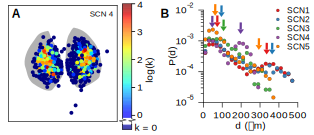
\includegraphics[height=1.5in]{fig5_new.pdf}
    \end{center}

    Small-world, bilateral symmetric, with hubs located in SCN central regions.\\\pause
    This does not perfectly correlate to a single known distribution of neurotransmitter expression. Which are involved?

\end{frame}


\begin{frame}{The role of VIP neurons in synchrony and entrainment}
    \footlineextra{Aton \textit{et al}. Nat Neurosci 2005}
    \begin{columns}
        \column{0.5\textwidth}
        One pathway likely driving this synchrony is VIP.\\[0.5em]

        \pause

    It is unknown how VIP is released endogenously, and how this is dependent upon electrical activity.
    \column{0.5\textwidth}

    \pause
    \fullpagegraphic{VIP.png}
    \end{columns}
\end{frame}

\begin{frame}{Study design: investigating role of VIP, electrical neurotransmission, and synchrony}

    Collaborator: Dr.\ Cristina Mazuski (Herzog lab)\pause

    \begin{enumerate}[<+->]
        \item Identify firing patterns in the SCN.
        \item Apply those patterns to VIP neurons via optogenetic stimulation.
        \item Characterize VIP release and circadian response.
    \end{enumerate}

    \footlineextra{Mazuski, Abel, Chen, Hermanstyne, Doyle, and Herzog, in revision}
\end{frame}

\begin{frame}{Recording from VIP and non-VIP SCN neurons}

        \includegraphics[height=1.2in]{expt_setup.png}\\\pause
        \includegraphics[height=1.2in]{expt_record.png}

    \footlineextra{Mazuski, Abel, Chen, Hermanstyne, Doyle, and Herzog, in revision}
\end{frame}


\begin{frame}{Identifying firing patterns in the SCN}

        \fullpagegraphic{mazuski2.png}

    \footlineextra{Mazuski, Abel, Chen, Hermanstyne, Doyle, and Herzog, in revision}
\end{frame}

\begin{frame}{Optogenetic stimulation triggers VIP release in a frequency-dependent fashion}

    \begin{columns}
        \column{0.5\textwidth}
    Apply optogenetic stimulation with constant rate at variable instantaneous frequency.\pause

    \fullpagegraphic{Figure3a.png}\pause

    \column{0.5\textwidth}
    VIP antagonist eliminates phase shift.

    \fullpagegraphic{Figure3c.png}
    \end{columns}
\end{frame}

\begin{frame}{Optogenetic stimulation of VIP neurons entrains circadian behavior in vivo via phase delays}
    \fullpagegraphic{entrainment.png}
    \footlineextra{Mazuski, Abel, Chen, Hermanstyne, Doyle, and Herzog, in revision}

\end{frame}


\begin{frame}{Conclusions: neurotransmission in the SCN}
    \begin{enumerate}
        \item Neurotransmission in the SCN relies on the confluence of numerous pathways and processes. 
            \begin{itemize}
                \item The central SCN is of importance within the small-world network. \pause
                \item VIP primarily evokes phase delays.\pause
                \item Neuropeptide release depends on electrical activity.\pause
            \end{itemize}
        \item Electrical activity: a fundamental component of the oscillator?
    \end{enumerate}
    \vspace{0.5em}

    \pause
    How does this relate to control? Control is the inverse problem.
\end{frame}

\nasasection{Controlling circadian rhythms}
\begin{frame}{The search for circadian pharmaceuticals}
    \begin{columns}
        \column{0.5\textwidth}

        {\it Potential uses:}
        \begin{itemize}
            \item resetting the clock
            \item "strengthening" oscillation
                \begin{itemize}
                    \item Robustness
                    \item Amplitude
                \end{itemize}
        \end{itemize}

        \column{0.5\textwidth}
        \fullpagegraphic{kl001_and_longdaysin.pdf}
    \end{columns}
    \footlineextra{Hirota \textit{et al.} Science 2012; St.~John \textit{et al.} PNAS 2014}
\end{frame}


\begin{frame}{The necessity of dynamic pharmaceutical dosing}
        \footlineextra{St.~John and Doyle PLoS Comp Bio 2015; Abel and Doyle Chem Eng Res Des 2016}

    {\it Traditional pharmaceuticals: phase-agnostic, long half-life}
    \begin{itemize}
        \item does not elicit a dynamic response (cannot reset the clock)
        \item drugs with transient effect discarded
    \end{itemize}

    \pause
    \vfill
    {\it Proposed approach: dynamic dosing}
    \begin{itemize}
        \item allows phase resetting due to transient stimulus
        \item utilize fast-acting drugs
    \end{itemize}
    \vspace{1em}
    \pause

    {\color{red}\it Challenge: drug application timing may result in drastically different responses.}


\end{frame}

\begin{frame}{Revisiting the mathematical formulation}

Consider the smooth dynamical system:
\begin{equation*}
    \label{eq:odes}
    \frac{dx}{dt} = f(x, p, u)
\end{equation*}
\pause

\vfill
The zero-input system has an exponentially attractive limit cycle, meaning
\begin{equation*}
    \label{eq:lc}
    \lim_{t\to\infty}[x(t) - x(t-T)]=0,
\end{equation*}

\pause
period: $T$\\
frequency: $\omega = \frac{2\pi}{T}$
\end{frame}






\begin{frame}{Development of the phase-reduced model}
    \footlineextra{Abel, Chakrabarty, and Doyle, in revision.}
    \begin{columns}
    \column{0.5\textwidth}
    \fullpagegraphic{phase_def.pdf}

        We can develop a phase-only formulation of the ODEs, by taking $\frac{d\hat\Phi}{dt}$.\pause
    \column{0.5\textwidth}


    Perform a first-order expansion of $\hat{\Phi}[\theta(t,x_a,u)]$ in $u$:

    \begin{equation*}
   \begin{split}
    \varphi(t,u) &= \hat{\Phi}[\theta(t,x_a,u)]\\
    \frac{d\varphi}{dt}&= \frac{d}{dt} \hat{\Phi}[\theta(t,x_a,u)]\\
    &= \omega + \underbrace{\frac{\partial}{\partial t}\frac{\partial\hat{\Phi}[\gamma(t,x_0)]}{\partial u}u(t)}_{\text{linear approx. in } u}
    \end{split}
\end{equation*}

\pause
Infinitesimal in both time and perturbation magnitude.
\end{columns}
\end{frame}

\begin{frame}{Development of the phase-reduced model}
\footlineextra{Taylor \textit{et al.} IEEE Trans Autom Control 2008; see Abel and Doyle, Chem Eng Res Des 2016 for calculation of ipPRC.}
We incorporate $u(t)$ into the ODE model as a time-dependent modification of parameters $p$:
\begin{equation*}
    p(t) = p_0+u(t)
\end{equation*}
so that $dp = du$.

\pause
Thus:
\begin{equation*}
    \label{eq:phiipprc}
    \boxed{\frac{d\varphi}{dt} = \omega + \frac{\partial}{\partial t}\frac{\partial\hat{\Phi}[\gamma(t,x_0)]}{\partial p}u(t),}
\end{equation*}
where $\frac{\partial}{\partial t}\frac{\partial\hat{\Phi}[\gamma]}{\partial p} = B(t)$ is the infinitesimal parametric phase response curve (ipPRC) for the oscillator on the limit cycle.
\end{frame}

\begin{frame}{Example: KL001 action}
    \fullpagegraphic{figure_1_kl001_actiona.png}
    \footlineextra{Mechanism: St.\ John \textit{et al.} PNAS 2014. Fig: Abel, Chakrabarty, and Doyle, in revision}
\end{frame}

\begin{frame}{Example: model reduction for phase control}

        \begin{block}{Full limit cycle model}

            8 material balances (ODEs), 21 kinetic parameters

            \includegraphics[width=0.8\textwidth]{equations.pdf}
        \end{block}

    \footlineextra{Abel, Chakrabarty, and Doyle, in revision.}
\end{frame}

\begin{frame}{Example: model reduction for phase control}

        \begin{block}{Effect of control input}
            Decrease in degradation rates for nuclear dimers.

\begin{equation*}
    \frac{d\mathrm{C1P}}{dt} = v_{\mathrm{a,{CP}}} \mathrm{P} \cdot \mathrm{C1} - v_{\mathrm{d,{ CP}}} \mathrm{C1P}  - \frac{{\color{red}( vdCn-u(t))} \mathrm{C1P} }{k_{\mathrm{deg,{Cn}}} +\mathrm{C1P}  + \mathrm{C2P} },
\end{equation*}
\begin{equation*}
    \frac{d\mathrm{C2P }}{dt} = v_{\mathrm{a,{CP}}} \mathrm{P}\cdot \mathrm{C2} - v_{\mathrm{d,{CP}}} \mathrm{C2P}- \frac{ {\color{red}(vdCn-u(t))} m_{\mathrm{C2N}} \mathrm{C2P} }{k_{\mathrm{deg,{Cn}}} + \mathrm{C2P}  +\mathrm{C1P} },
\end{equation*}

        \end{block}

    \footlineextra{Abel and Doyle, Chem Eng Res Des 2016}
\end{frame}

\begin{frame}{Example: model reduction for phase control}

        \begin{block}{Effect of control input}
            Calculate the phase sensitivity to yield the phase only formulation:

            \begin{equation*}
            \frac{d\varphi}{dt} = \omega + B(\varphi)\cdot u(t)
            \end{equation*}

            and

\begin{equation*}
    B(\varphi) = -\frac{\partial}{\partial t}\frac{\partial\hat\Phi[\gamma(t,x_0)]}{d({vdCn})}
\end{equation*}

where $B(\varphi)$ is the KL001 ipPRC.
        \end{block}

    \footlineextra{Abel, Chakrabarty, and Doyle, in revision.}
\end{frame}

\begin{frame}{ipPRC calculation}
    \fullpagegraphic{figure_1_kl001_action.png}
    \footlineextra{Abel, Chakrabarty, and Doyle, Proc. 20th IFAC World Congress 2017.}
\end{frame}

\begin{frame}{The phase resetting problem}
    \footlineextra{Abel, Chakrabarty, and Doyle, in revision.}
    \begin{alertblock}{Oscillator:}
        \[\frac{d\varphi}{dt} =  \omega + B(\varphi)\cdot u(t), \;\; \varphi(0)=\phi_0\]
    \end{alertblock}
    \pause
     \begin{alertblock}{Environment:}
        \[
            \frac{d\varphi_r}{dt} =  \omega_r + \Delta\phi_f \delta(t_{shift})
            \;\; \varphi_r(0)=\phi_0
        \]
    \end{alertblock}
    \pause

     \begin{alertblock}{Phase error:}
        \[
            \chi(t) = \varphi(t)-\varphi_r(t) \; \mod2\pi
        \]
    \end{alertblock}
     The terminal condition is $\chi(t_f)=0$. We want to reach this in minimum time.


\end{frame}



\begin{frame}{Optimal phase shifting: fixed endpoint, free time}

    State dynamics:
    \begin{align}
        \dot\varphi &= \omega + B(\varphi)\cdot u(t) \tag{ODE}\\
        \nonumber\varphi(0) &= \varphi_0
    \end{align}\pause

    Cost functional:
    \begin{equation}\tag{J}
        J[u(t)] = \int_0^{t_f} 1\,dt
    \end{equation}\pause

    Hamiltonian:
    \begin{equation}\tag{H}
        H(\varphi,\lambda,u) = (\omega+B(\varphi)\cdot u)\cdot\lambda -1
    \end{equation}
\end{frame}

\begin{frame}{Pontryagin's maximum principle}
    Maximization condition:
    \begin{align}\tag{M}
        H(\varphi,\lambda,u) &= \max_{u_{\min}\leq u\leq u_{\max}}\{(\omega+B(\varphi)\cdot u)\cdot\lambda -1\}\\
        \nonumber &= \omega\cdot\lambda - 1+ \max_{u_{\min}\leq u\leq u_{\max}}\{B(\varphi)\cdot u \cdot\lambda\}
    \end{align}

    \pause
    Thus, the control law is:
    \begin{equation*}
    u^\star(t) = \begin{cases}u_{\max} &\mbox{if } B(\varphi)\cdot\lambda >0 \\
        u_{\min} & \mbox{if }B(\varphi)\cdot\lambda \leq0 \end{cases}
    \end{equation*}
    which is {\bf bang-bang control}.

    \pause
    The terminal condition $\lambda(t_f) = 0$, so costate $\lambda$ will ever only be either positive or negative. Thus {\bf control input for a specific case depends only on} ${\rm sgn}(B(\varphi))$.

    \footlineextra{Similar result shown for limit cycle model: Zhang, Qiao, Julius Automatica 2016}
\end{frame}

\begin{frame}{Optimal control inputs}
For an oscillator with desired phase shift $\Delta\varphi_f$, starting at phase $\varphi(0) = \phi_0$, the optimal control input is that for achieving either the positive phase shift:
\begin{equation*}
    u^{+}(t) = \begin{cases}u_{\max} &\mbox{if } B(\varphi) >0 \\
        u_{\min} & \mbox{if } B(\varphi) \leq0 \end{cases}
\end{equation*}
or the negative phase shift:
\begin{equation*}
    u^{-}(t) = \begin{cases}u_{\max} &\mbox{if } B(\varphi) <0 \\
        u_{\min} & \mbox{if } B(\varphi) \geq0 \end{cases}.
\end{equation*}

\footlineextra{Abel, Chakrabarty, and Doyle, in revision.}

\end{frame}



\begin{frame}
    \frametitle{Example: optimal phase shifting}
    Either \textbf{delay} or advance, \it{not both}

    \pause
    \fullpagegraphic{delay.png}

\end{frame}
\begin{frame}[noframenumbering]
    \frametitle{Example: optimal phase shifting}
    Either delay or \textbf{advance}, \it{not both}

    \fullpagegraphic{advance.png}

\end{frame}

\begin{frame}
    \frametitle{A bound on the time to reset phase}
    Where these shifts meet is the most "distant" phase.

    \fullpagegraphic{upperlimit.png}
\end{frame}

\begin{frame}
    \frametitle{Optimal control law for any shift}
    \fullpagegraphic{directionselection.png}

    Also allows identification of optimal direction of phase shifting.
\end{frame}

\begin{frame}{Application for model predictive control}
        MPC is a form of feedback control where control is changed at discrete steps based on an optimization of predicted trajectory.\\\pause
    \fullpagegraphic{figure_2.png}

    \pause
    Not shown: bounding error between optimal and model predictive control (Abel, Chakrabarty, and Doyle, in revision).
\end{frame}

\begin{frame}{MPC applied in silico for jet lag}
    \fullpagegraphic{figure_7.png}
    \footlineextra{Abel, Chakrabarty, and Doyle, in revision.}
\end{frame}

\begin{frame}{MPC applied in silico for rotating shift work}
    \fullpagegraphic{figure_8.png}
    \footlineextra{Abel, Chakrabarty, and Doyle, in revision.}

    Schedule from Vetter \textit{et al.}, Curr Biol 2015.
\end{frame}



\begin{frame}{Conclusions: control of circadian rhythms}
    \begin{enumerate}
        \item Control theory has a useful toolkit to offer for manipulating dynamic biological processes.\pause
        \item We have established useful bounds on effectiveness of pharmaceuitcal circadian resetting.\pause
            \begin{itemize}
                \item Lower bounds on time to reset for a given drug.\pause
                \item Upper bounds on error from MPC implementation.
            \end{itemize}
    \end{enumerate}
\end{frame}


\begin{frame}{Future study: control of circadian rhythms}
    \begin{columns}
        \column{0.4\textwidth}
    \begin{enumerate}
        \item Develop techniques for phase inference to close the loop\pause
        \item Apply MPC controllers to SCN or peripheral oscillator cultures (proposal pending)\pause
        \item Population control
    \end{enumerate}
    \column{0.6\textwidth}
    \pause
    \fullpagegraphic{fig4_population.png}
    \end{columns}
\end{frame}

\begin{frame}{Future study: more challenging methods}
        Critical resetting: targeting the limit cycle fixed point where all phases coexist. \pause

    \fullpagegraphic{ctrl.png}
\end{frame}

\metroset{background=dark}
\section*{Acknowledgment}
\metroset{background=light}

\begin{frame}[noframenumbering]
    \frametitle{Acknowledgments: Formal Affiliations}
    {\footnotesize
    \begin{columns}
        \column{0.5\textwidth}
        {\it Collaborator + Committee Member}

    Prof. Erik Herzog (WUSTL)

    {\it DAC \& Committee}\\
    Prof. Johan Paulsson\\
    Prof. Galit Lahav\\
    Prof. John Higgins\\
    Prof. Charles Czeisler

    \column{0.5\textwidth}
    {\it Co-advisors}

    Prof. Linda Petzold (UCSB)\\
    Prof. Elizabeth Klerman (HMS/BWH)
    \end{columns}

    \vspace{0.3cm}

    \begin{columns}
        \column{0.45\textwidth}
    Doyle lab, Harvard University\\
    \includegraphics[height = 3.cm]{doylelab.jpg}

    \column{0.5\textwidth}
    AMU, Brigham and Women's Hospital\\
    \includegraphics[height = 3.cm]{amu.jpg}
    \end{columns}

    \vfill
    {\it Funding and affiliations:}\hspace{0.5cm}
    \includegraphics[height=1cm]{nih.png}\hspace{0.5cm}
    \includegraphics[height=1cm]{hms.png}\hspace{0.5cm}
    \includegraphics[height=1cm]{bwh.png}\\
    \scriptsize{NIH T32-HLO7901, Training Program in Sleep, Circadian, \& Respiratory Neurobiology}}
\end{frame}

\begin{frame}[noframenumbering]
    \frametitle{Acknowledgments II: Direct Collaborators}
    {\footnotesize
    \begin{columns}
        \column{0.5\textwidth}
        {\it Doyle lab}\\
        Dr. Peter St.\ John\\
        Dr. Ankush Chakrabarty\\
        Kelsey Dean\\
        Lindsey Brown

        {\it Herzog lab}\\
        Dr. Daniel Granados-Fuentes\\
        Dr. Vania Carmona-Alcocer\\
        Dr. Cristina Mazuski

        {\it Petzold lab}\\
        Dr. Brian Drawert

        {\it Klerman lab/BWH}\\
        Dr. Amene Asgari\\
        Dr. Andrew J.K. Phillips

        {\it Takahashi lab}\\
        Dr. Yongli Shan

        \column{0.5\textwidth}

        \fullpagegraphic{herzoglab.png}

        \fullpagegraphic{hike.jpg}
    \end{columns}
    }
\end{frame}

\begin{frame}[noframenumbering]
    \frametitle{Acknowledgments III}
    {\footnotesize
    \begin{columns}
        \column{0.5\textwidth}

        UCSB\\[1em]

        Harvard\\
        Liz Pomerantz and Sam Reed\\
        Evi and Ivana\\[1em]
        Tufts\\
        Prof. Hyunmin Yi\\
        Dr. Sukwon Jung\\[1em]
        Faith Blake\\
        Anthony Abel\\
        Community/Friends/Family

        \column{0.5\textwidth}


        \fullpagegraphic{ucsb.jpg}

        \fullpagegraphic{tufts.jpg}




    \end{columns}
    }
\end{frame}

\metroset{background=dark}
\begin{frame}[noframenumbering]

    \emph{\bf{\huge{Open questions?}}}

\end{frame}
\metroset{background=light}


\end{document}










